% !TEX program = xelatex
\documentclass[9pt, aspectratio=169]{beamer}
\usetheme{metropolis}
\usefonttheme{professionalfonts}

% --- Modern Font Setup ---
\usepackage[T1]{fontenc}
\usepackage{FiraSans}  % Modern, elegant sans-serif font family
\usepackage[scaled=0.95]{FiraMono}  % Matching monospace font

% Lighter, more refined font weights
\renewcommand{\seriesdefault}{l}  % Light weight as default
\renewcommand{\bfseries}{\fontseries{sb}\selectfont}  % Semi-bold instead of bold

% Custom font sizing - more refined
\setbeamerfont{title}{size=\Large, series=\fontseries{m}\selectfont}
\setbeamerfont{subtitle}{size=\normalsize, series=\fontseries{l}\selectfont}
\setbeamerfont{author}{size=\small, series=\fontseries{l}\selectfont}
\setbeamerfont{date}{size=\small, series=\fontseries{l}\selectfont}
\setbeamerfont{frametitle}{size=\normalsize, series=\fontseries{m}\selectfont}
\setbeamerfont{framesubtitle}{size=\footnotesize, series=\fontseries{l}\selectfont}
\setbeamerfont{block title}{size=\normalsize, series=\fontseries{m}\selectfont}
\setbeamerfont{block body}{size=\small}
\setbeamerfont{itemize/enumerate body}{size=\small}
\setbeamerfont{itemize/enumerate subbody}{size=\footnotesize}
\setbeamerfont{section in toc}{size=\normalsize, series=\fontseries{m}\selectfont}
\setbeamerfont{section title}{size=\Large, series=\fontseries{m}\selectfont}

% --- Color Definitions ---
% Primary Theme Colors
\definecolor{PrimaryColor}{RGB}{33,52,72}         % Deep navy
\definecolor{SecondaryColor}{RGB}{84,119,146}     % Desaturated blue-gray
\definecolor{AccentColor}{RGB}{100,156,165}       % Soft steel blue
\definecolor{black}{RGB}{0,0,0}
\definecolor{BackgroundColor}{RGB}{245,247,250}   % Very light cool gray/blue-tinted white
\definecolor{TextColor}{RGB}{40,55,70}            % Darker, cool-toned charcoal
\definecolor{LightGray}{RGB}{220,225,230}         % Soft, cool light gray
\definecolor{DarkGray}{RGB}{70,90,105}            % Cool-toned dark gray

% --- Theme Customization ---
\setbeamercolor{background canvas}{bg=BackgroundColor}
\setbeamercolor{normal text}{fg=TextColor}
\setbeamercolor{frametitle}{bg=PrimaryColor, fg=white}
\setbeamercolor{section in toc}{fg=PrimaryColor}
\setbeamercolor{block title}{bg=PrimaryColor!80, fg=white}
\setbeamercolor{block body}{bg=PrimaryColor!10}
\setbeamercolor{alerted text}{fg=AccentColor}
\setbeamercolor{itemize item}{fg=PrimaryColor}
\setbeamercolor{itemize subitem}{fg=SecondaryColor}

% Progress bar
\setbeamercolor{progress bar}{fg=AccentColor, bg=LightGray}

% --- Packages ---
\usepackage[utf8]{inputenc}
\usepackage{url}
\usepackage{booktabs}
\usepackage{amsmath, amssymb, amsfonts}
\usepackage{fontawesome5}
\usepackage{pifont}
\usepackage[most]{tcolorbox}
\tcbuselibrary{skins, listings}
\usepackage{colortbl}
\usepackage{array}
\usepackage{adjustbox}
\usepackage{ragged2e}

% --- Packages for plotting discrete and continuous signals and spectrums ---
\usepackage{tikz}
\usepackage{circuitikz} % Useful for signal processing block diagrams
\usepackage{pgfplots}
\usepackage{graphicx}
\usepackage{caption}
\usepackage{subcaption}

\usetikzlibrary{shapes.callouts, positioning, arrows.meta, shapes.geometric, shadows, calc, patterns, backgrounds, shadings, fit, chains, decorations.pathreplacing, intersections}
\usepgfplotslibrary{fillbetween}
\usepgfplotslibrary{polar}
\pgfplotsset{compat=1.18}
\pgfplotsset{
    plot coordinates/math parser=false,
    signal/.style={thick, color=PrimaryColor},
    spectrum/.style={thick, color=AccentColor},
    discrete/.style={ycomb, mark=*, mark options={fill=white, draw=PrimaryColor}, color=PrimaryColor, thick},
}

% --- Custom Commands ---
\newcommand{\cmark}{\textcolor{PrimaryColor}{\ding{51}}}
\newcommand{\xmark}{\textcolor{AccentColor}{\ding{55}}}
\newcommand{\highlight}[1]{\textcolor{PrimaryColor}{\textbf{#1}}}

% --- Custom tcolorbox environments ---
\newtcolorbox{conceptbox}[1]{
    colback=PrimaryColor!10,
    colframe=PrimaryColor,
    title=#1,
    fonttitle=\small\bfseries,
    fontupper=\small,
    rounded corners
}

\newtcolorbox{insightbox}[1]{
    colback=AccentColor!10,
    colframe=AccentColor,
    title=#1,
    fonttitle=\small\bfseries,
    fontupper=\small,
    rounded corners
}

\newtcolorbox{algorithmbox}[1]{
    colback=SecondaryColor!10,
    colframe=SecondaryColor,
    title=#1,
    fonttitle=\small\bfseries,
    fontupper=\small,
    rounded corners
}

\newtcblisting{codelistingbox}[2][]{
    colback=SecondaryColor!10,
    colframe=SecondaryColor,
    title=#2,
    fonttitle=\small\bfseries,
    rounded corners,
    listing only,
    listing options={
            language=#1,
            basicstyle=\ttfamily\footnotesize,
            keywordstyle=\color{PrimaryColor}\bfseries,
            commentstyle=\color{SecondaryColor}\itshape,
            stringstyle=\color{AccentColor},
            numbers=left,
            numberstyle=\tiny\color{DarkGray},
            stepnumber=1,
            showstringspaces=false,
            tabsize=4
        }
}


\subtitle{Signals and Linear Systems}
\date{}
\author{Ashrafur Rahman\\Lecturer, CSE, BUET}
\institute{ashrafur@cse.buet.ac.bd}


\title{The Fast Fourier Transform}

\begin{document}

\maketitle

\begin{frame}{Outline}
    \begin{itemize}
        \item \textbf{Recap of Last Class}
        \item \textbf{The Need for Speed:} Naive DFT complexity
        \item \textbf{Fast Fourier Transform (FFT):}
              \begin{itemize}
                  \item Radix-2 Decimation-in-Time (DIT)
                  \item Radix-2 Decimation-in-Frequency (DIF)
              \end{itemize}
        \item \textbf{Conclusion:} FFT Complexity Analysis
    \end{itemize}
\end{frame}

\begin{frame}{Recap of Last Class}
    \begin{itemize}
        \item In the last class we derived and looked at the DFT from 2 different perspectives.
              \begin{itemize}
                  \item \textbf{Periodic:}
                        \begin{itemize}
                            \item DFT can be viewed as the evaluation of the Fourier series coefficients of a \emph{sampled} periodic signal.
                            \item It can also be viewed as the $N$ unique values of the fourier series of a discrete-time periodic signal.
                        \end{itemize}
                  \item \textbf{Aperiodic:}
                        \begin{itemize}
                            \item DFT can be viewed as samples of the continuous-time Fourier transform of a \emph{sampled} aperiodic signal.
                            \item It can also be viewed as samples of the discrete-time fourier transform of a finite-length sequence.
                        \end{itemize}
                  \item As we will see later, if the original conginuous signal is bandlimited, we can recover the original signal from the DFT.
              \end{itemize}
    \end{itemize}
\end{frame}

\begin{frame}{Naive Evaluation of the DFT}
    Now let's go into the computational complexity of evaluating the DFT.
    \begin{itemize}
        \item Let's examine the computational complexity of evaluating the DFT directly from its definition:
              \begin{equation*}
                  X[k] = \sum_{n=0}^{N-1} x[n]W_N^{kn}, \qquad \text{where } W_N = e^{-j\frac{2\pi}{N}}
              \end{equation*}
        \item For each of the $N$ values of $k$, we must compute:
              \begin{itemize}
                  \item $N$ complex multiplications
                  \item $N-1$ complex additions
              \end{itemize}
        \item Therefore, calculating all $N$ values of $X[k]$ explicitly requires \textbf{$O(N^2)$} operations.
        \item \textbf{Why is this a problem?}
              \begin{itemize}
                  \item Consider 1 second of audio sampled at 44.1 kHz. Here, $N = 44,100$.
                  \item The naive DFT requires roughly $N^2 \approx 2 \times 10^9$ operations!
                        This would make spectral analysis impossibly slow.
              \end{itemize}
    \end{itemize}
\end{frame}

\begin{frame}{A Brief History of the FFT}
    \begin{columns}[T] % [T] aligns columns at the top
        \begin{column}{0.6\textwidth}
            \begin{itemize}
                \item \textbf{1805: Carl Friedrich Gauss}
                      \begin{itemize}
                          \item Developed the radix-2 algorithm to interpolate asteroid orbits.
                          \item Predates Joseph Fourier's work on harmonic analysis by over a decade!
                          \item Left it as a note, unpublished.
                      \end{itemize}
                      \vspace{1.2cm} % Adjust space to align text with images
                \item \textbf{1965: James Cooley \& John Tukey}
                      \begin{itemize}
                          \item Independently rediscovered the algorithm at IBM and Princeton.
                          \item Their landmark paper launched the modern field of Digital Signal Processing (DSP).
                      \end{itemize}
                \item Many other variants of the FFT have been developed since then. But we are going to study the Cooley-Tukey FFT first.
            \end{itemize}
        \end{column}

        \begin{column}{0.25\textwidth}
            \centering
            \vspace{-0.3cm}

            \begin{figure}
                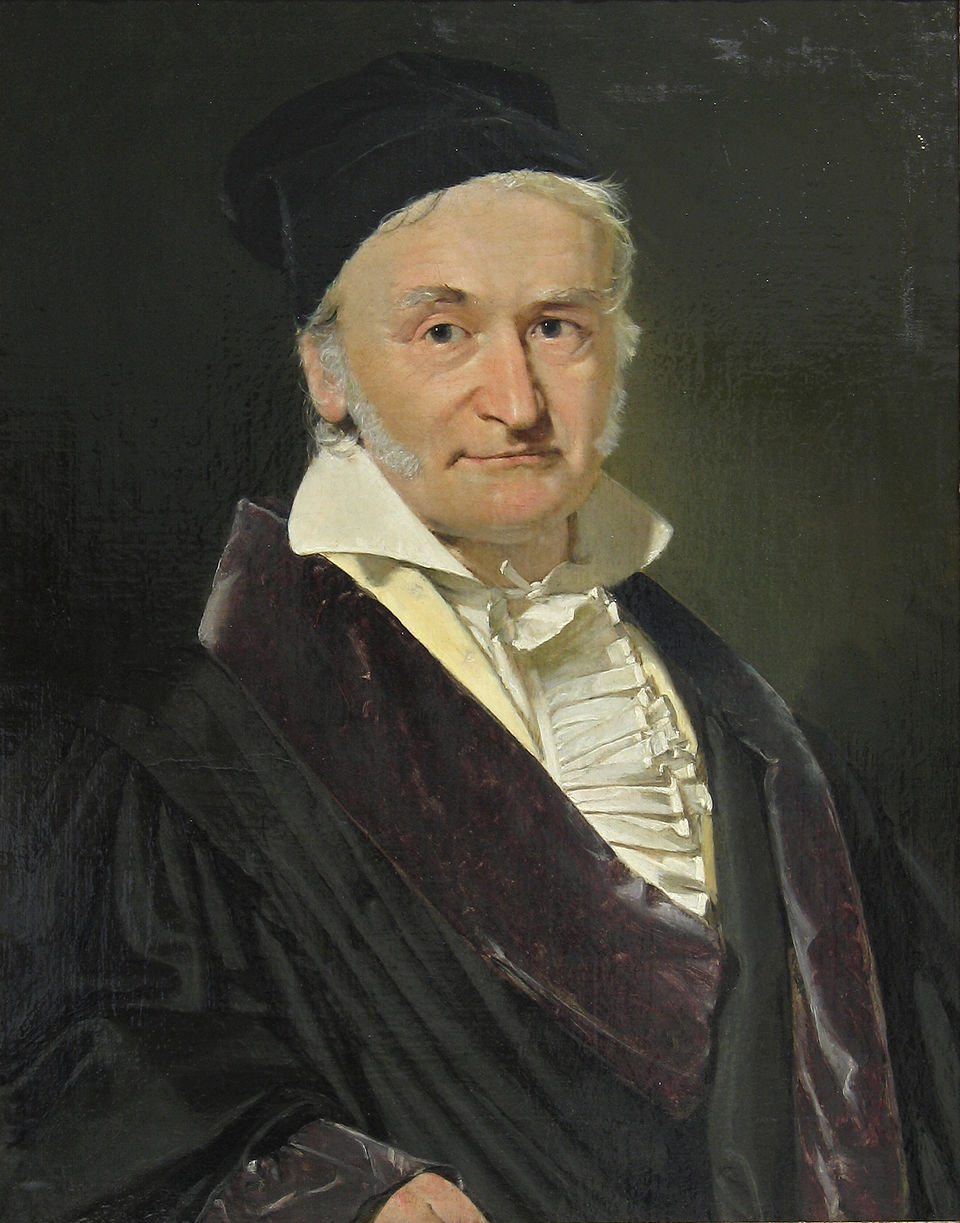
\includegraphics[width=0.55\textwidth, height=2.5cm, keepaspectratio]{figures/gauss.jpg}
                \vspace{-0.1cm}
                \caption*{\scriptsize Carl Friedrich Gauss}
            \end{figure}

            \begin{minipage}{0.48\textwidth}
                \centering
                
\includegraphics[width=\textwidth, height=2.0cm, keepaspectratio]{figures/cooley.jpg}
                \captionof*{figure}{\scriptsize James W. Cooley}
            \end{minipage}
            \hfill
            \begin{minipage}{0.48\textwidth}
                \centering
                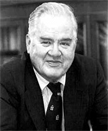
\includegraphics[width=\textwidth, height=2.0cm, keepaspectratio]{figures/tukey.jpg}
                \captionof*{figure}{\scriptsize John W. Tukey}
            \end{minipage}
        \end{column}
    \end{columns}
\end{frame}

\begin{frame}{Cooley-Tukey FFT Algorithm}
    \begin{itemize}
        \item The Cooley-Tukey FFT Algorithm is an elegant $O(N \log N)$ algorithm to compute the DFT by exploiting the symmetry and periodicity of $W_N$.
              Recall the DFT definition:
              \begin{align*}
                  X[k] & = \sum_{n=0}^{N-1} x[n]W_N^{kn} \qquad \text{where } W_N = e^{-j\frac{2\pi}{N}}
              \end{align*}
        \item We are first going to study the \textbf{radix-2} FFT algorithm
              which--
              \begin{itemize}
                  \item Successively splits an $N$-point DFT into two $N/2$-point DFTs.
                  \item Assumes $N$ is a power of 2 (if not, use zero-padding).
              \end{itemize}
        \item There are two variants of the Cooley-Tukey FFT algorithm:
              \begin{itemize}
                  \item \textbf{Decimation-in-Time (DIT)}
                  \item \textbf{Decimation-in-Frequency (DIF)}
              \end{itemize}
    \end{itemize}
\end{frame}

\begin{frame}{Decimation-in-Time (DIT) FFT}
    \begin{itemize}
        \item \textbf{Decimation-in-Time} splits the time-domain sequence $x[n]$ into its \textbf{even} and \textbf{odd} indexed samples:
              \begin{align*}
                  X[k] & = \sum_{n=0}^{N-1} x[n]W_N^{kn} = \sum_{r=0}^{N/2-1} x[2r]W_N^{2rk} + \sum_{r=0}^{N/2-1} x[2r+1]W_N^{(2r+1)k}
              \end{align*}
        \item Since $W_N^{2rk} = e^{-j\frac{2\pi}{N}2rk} = e^{-j\frac{2\pi}{N/2}rk} = W_{N/2}^{rk}$, we get:
              \begin{align*}
                  X[k] & = \underbrace{\sum_{r=0}^{N/2-1} x[2r]W_{N/2}^{rk}}_{\text{$N/2$-point DFT of evens}} + W_N^k \underbrace{\sum_{r=0}^{N/2-1} x[2r+1]W_{N/2}^{rk}}_{\text{$N/2$-point DFT of odds}}
              \end{align*}
        \item So, we can compute the $N$-point DFT $X[k]$ by computing two $N/2$-point DFTs!
        \item But we need some way to convert the $N/2$-point DFTs to $N$-points.
    \end{itemize}
\end{frame}

\begin{frame}{Decimation-in-Time (DIT) FFT (cont.)}
    \begin{itemize}
        \item Define new functions:
              \begin{align*}
                  G[k] & = \sum_{r=0}^{N/2-1} x[2r]W_{N/2}^{rk} = \text{DFT}\{x[2r] \text{ with } N/2 \text{ points}\}     \\
                  H[k] & = \sum_{r=0}^{N/2-1} x[2r+1]W_{N/2}^{rk} = \text{DFT}\{x[2r+1] \text{ with } N/2 \text{ points}\}
              \end{align*}
        \item $G[k]$ and $H[k]$ is clearly defined for $0 \le k < N/2$.
        \item But also since $N/2$-point DFT is periodic with period $N/2$, we have:
              \begin{align*}
                  G[k + N/2] & = G[k] \\
                  H[k + N/2] & = H[k]
              \end{align*}

        \item So if we copy the first half of $G[k]$ and $H[k]$ to the second half (periodic extension), we can write:
              \begin{align*}
                  X[k] & = G[k] + W_N^k H[k]
              \end{align*}
        \item However, we can do better.
    \end{itemize}
\end{frame}

\begin{frame}{Decimation-in-Time (DIT) FFT (cont.)}
    \begin{itemize}
        \item For the second half, $N/2 \le k < N$, we can use the property $W_N^{k+N/2} = W_N^k e^{-j\pi} = -W_N^k$:
              \begin{align*}
                  X[k + N/2] & = G[k + N/2] + W_N^{k+N/2} H[k + N/2]                 \\
                             & = G[k] - W_N^k H[k] \qquad \text{ for } N/2 \le k < N
              \end{align*}

        \item So, together we can write:
    \end{itemize}
    \begin{conceptbox}{Radix-2 Decimation-in-Time FFT}
        For $0 \le k < N/2$:
        \begin{align*}
            X[k]       & = G[k] + W_N^k H[k] \\
            X[k + N/2] & = G[k] - W_N^k H[k]
        \end{align*}
    \end{conceptbox}
    \begin{itemize}
        \item This means we only need to compute the $N/2$-point DFTs of the even and odd parts once, and then combine them using simple additions/subtractions and a single complex multiplication (the \textbf{"twiddle factor"}) for each output.
    \end{itemize}
\end{frame}

\begin{frame}{DIT Butterfly Structure ($N=2$)}
    Now let us see the computational structure of the FFT by walking through for small values of $N$.

    \vspace{1cm}
    \begin{minipage}{0.48\textwidth}
        \begin{itemize}
            \item The fundamental operation is the 2-point DFT (butterfly).
            \item Note that $W_2^0 = 1$.
        \end{itemize}
        \vspace{0.4cm}
        \begin{align*}
            X[0] & = x[0] + x[1]W_2^0 = x[0] + x[1] \\
            X[1] & = x[0] - x[1]W_2^0 = x[0] - x[1]
        \end{align*}
    \end{minipage}
    \hfill
    \begin{minipage}{0.48\textwidth}
        \begin{center}
            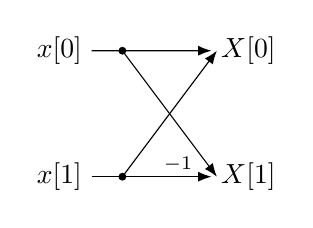
\begin{tikzpicture}[>=Latex, scale=0.8]
                \node (x0) at (0, 2) {$x[0]$};
                \node (x1) at (0, 0) {$x[1]$};
                \node (X0) at (3, 2) {$X[0]$};
                \node (X1) at (3, 0) {$X[1]$};

                \draw[->] (x0) -- (X0);
                \draw[->] (x1) -- (X1);

                \draw[->] (1.0,0) -- (2.5,2);
                \draw[->] (1.0,2) -- node[pos=0.8, below left=-2pt, font=\scriptsize] {$-1$} (2.5,0);

                \filldraw (1.0,2) circle (1.5pt);
                \filldraw (1.0,0) circle (1.5pt);
            \end{tikzpicture}
        \end{center}
    \end{minipage}
\end{frame}

\begin{frame}{DIT Butterfly Structure ($N=4$)}
    \begin{minipage}{0.48\textwidth}
        \begin{itemize}
            \item A 4-point DFT is built from two 2-point DFTs.
            \item $G[k]$ and $H[k]$ (outputs of Stage 1) are combined using twiddle factors $W_4^k$.
        \end{itemize}
        \vspace{0.2cm}
        \textbf{Explicit Formula:}
        \vspace{-0.2cm}
        \begin{align*}
            X[0] & = G[0] + W_4^0 H[0] \\
            X[1] & = G[1] + W_4^1 H[1] \\
            X[2] & = G[0] - W_4^0 H[0] \\
            X[3] & = G[1] - W_4^1 H[1]
        \end{align*}
    \end{minipage}
    \hfill
    \begin{minipage}{0.48\textwidth}
        \begin{center}
            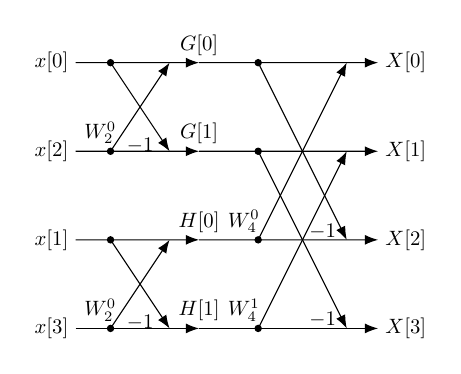
\begin{tikzpicture}[>=Latex, scale=0.75, transform shape]
                % Inputs
                \node (x0) at (0, 4.5) {$x[0]$};
                \node (x2) at (0, 3.0) {$x[2]$};
                \node (x1) at (0, 1.5) {$x[1]$};
                \node (x3) at (0, 0.0) {$x[3]$};

                % Outputs
                \node (X0) at (6, 4.5) {$X[0]$};
                \node (X1) at (6, 3.0) {$X[1]$};
                \node (X2) at (6, 1.5) {$X[2]$};
                \node (X3) at (6, 0.0) {$X[3]$};

                % Stage 1
                \draw[->] (x0) -- (2.5, 4.5);
                \draw[->] (x2) -- (2.5, 3.0) node[pos=0.2, above] {$W_2^0$};
                \draw[->] (x1) -- (2.5, 1.5);
                \draw[->] (x3) -- (2.5, 0.0) node[pos=0.2, above] {$W_2^0$};

                \draw[->] (1,0.0) -- (2.0, 1.5);
                \draw[->] (1,1.5) -- node[pos=0.8, below left=-2pt] {$-1$} (2.0, 0.0);
                \draw[->] (1,3.0) -- (2.0, 4.5);
                \draw[->] (1,4.5) -- node[pos=0.8, below left=-2pt] {$-1$} (2.0, 3.0);

                \filldraw (1,4.5) circle(1.5pt) (1,3.0) circle(1.5pt) (1,1.5) circle(1.5pt) (1,0) circle(1.5pt);

                % Stage 2
                \draw[->] (2.5, 4.5) -- node[pos=0, above] {$G[0]$} (X0);
                \draw[->] (2.5, 3.0) -- node[pos=0, above] {$G[1]$} (X1);
                \draw[->] (2.5, 1.5) -- node[pos=0, above] {$H[0]$} (X2) node[pos=0.25, above] {$W_4^0$} node[pos=0.69, yshift=-3pt, above] {$-1$};
                \draw[->] (2.5, 0.0) -- node[pos=0, above] {$H[1]$} (X3) node[pos=0.25, above] {$W_4^1$} node[pos=0.69, yshift=-3pt, above] {$-1$};

                \draw[->] (3.5, 1.5) -- (5, 4.5);
                \draw[->] (3.5, 0.0) -- (5, 3.0);
                \draw[->] (3.5, 4.5) -- (5, 1.5);
                \draw[->] (3.5, 3.0) -- (5, 0.0);

                \filldraw (3.5,4.5) circle(1.5pt) (3.5,3.0) circle(1.5pt) (3.5,1.5) circle(1.5pt) (3.5,0) circle(1.5pt);
            \end{tikzpicture}
        \end{center}
    \end{minipage}
\end{frame}

\begin{frame}{DIT 8-Point FFT: First Iteration}
    \begin{itemize}
        \item For $N=8$, the sequence is split into $N/2=4$-point DFTs of even and odd indices.
        \item The outputs $G(k)$ (evens) and $H(k)$ (odds) are combined using the relation:
        \item $X[k] = G(k) + W_8^k H(k)$ and $X(k+4) = G(k) - W_8^k H(k)$ for $k=0,\dots,3$.
    \end{itemize}
    \vspace{0.2cm}
    \begin{center}
        \begin{figure}
            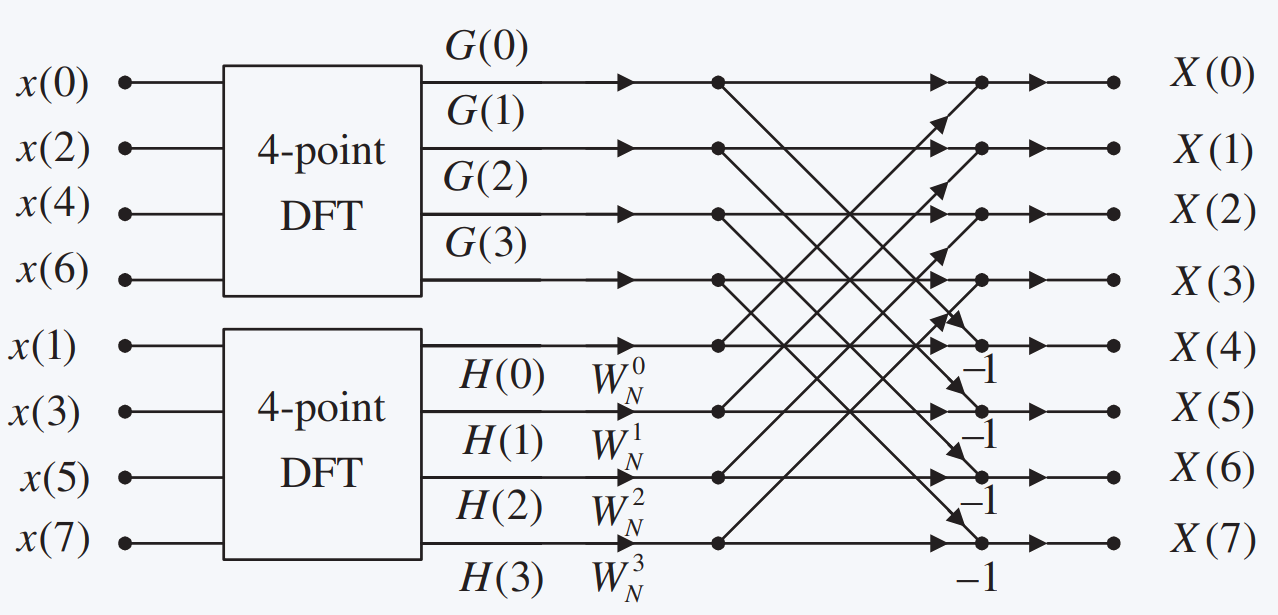
\includegraphics[width=0.6\textwidth]{figures/dit1.png}
        \end{figure}
    \end{center}
\end{frame}

\begin{frame}{DIT 8-Point FFT: Full Algorithm}
    \begin{itemize}
        \item Expanding all 4-point and 2-point DFTs yields the complete 8-point DIT structure.
        \item Notice the inputs are in \textbf{bit-reversed} order, while outputs are in \textbf{natural} order.
    \end{itemize}
    \vspace{0.2cm}
    \begin{center}
        \begin{figure}
            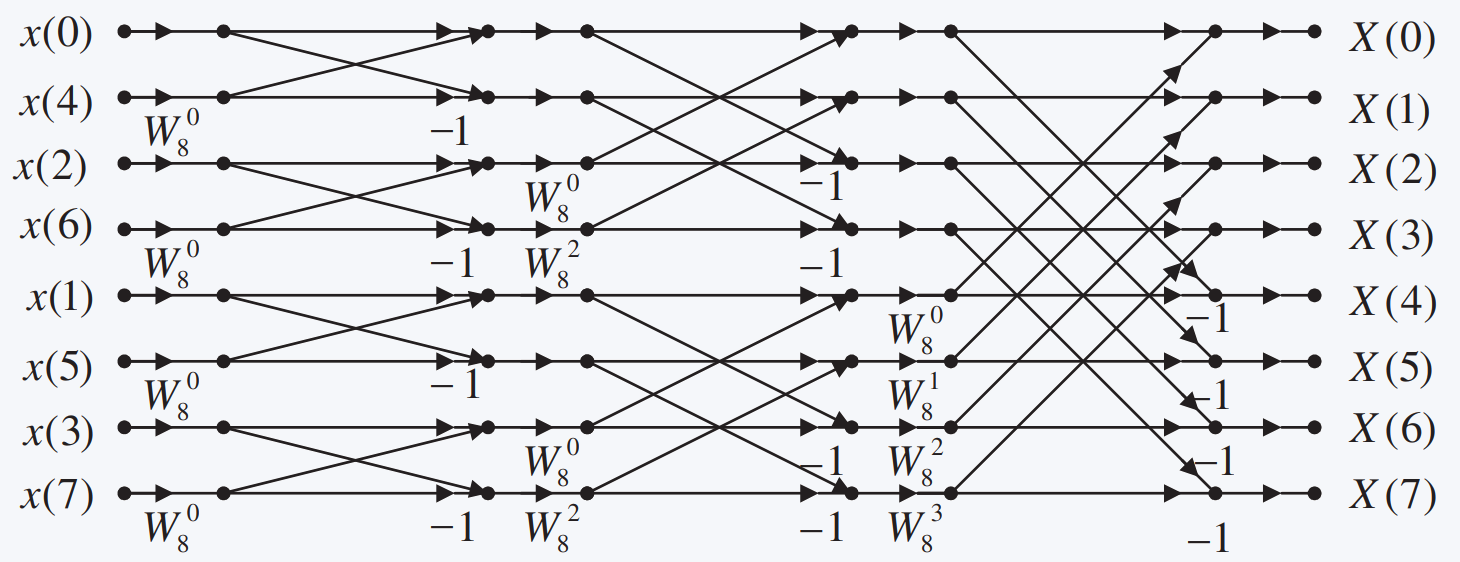
\includegraphics[width=0.7\textwidth]{figures/dit2.png}
        \end{figure}
    \end{center}
\end{frame}

\begin{frame}{Understanding Bit-Reversed Order}
    \begin{itemize}
        \item In Radix-2 DIT FFT, the inputs appear in \textbf{bit-reversed} order.
        \item Why? The sequence is successively divided into even and odd indexed halves.
        \item For $N=8$, the physical movements happen in three stages:
              \begin{enumerate}
                  \item \textbf{Stage 1:} Even (0,2,4,6), Odd (1,3,5,7)
                  \item \textbf{Stage 2:} Even-Even (0,4), Odd-Even (2,6), Even-Odd (1,5), Odd-Odd (3,7)
                  \item \textbf{Stage 3:} Single elements: $x[0], x[4], x[2], x[6], x[1], x[5], x[3], x[7]$
              \end{enumerate}
    \end{itemize}
    \begin{center}
        \scriptsize
        \begin{tabular}{cccc}
            \toprule
            Original Index & Binary & Bit-Reversed Binary & New Position \\
            \midrule
            $0$            & $000$  & $000$               & $0$          \\
            $1$            & $001$  & $100$               & $4$          \\
            $2$            & $010$  & $010$               & $2$          \\
            $3$            & $011$  & $110$               & $6$          \\
            $4$            & $100$  & $001$               & $1$          \\
            $5$            & $101$  & $101$               & $5$          \\
            $6$            & $110$  & $011$               & $3$          \\
            $7$            & $111$  & $111$               & $7$          \\
            \bottomrule
        \end{tabular}
    \end{center}
    \begin{itemize}
        \item Putting even before odd corresponds to sorting by the rightmost bit.
        \item Putting even-even before odd-even corresponds to sorting by the second rightmost bit, and so on.
        \item This is equivalent to sorting the input sequence by the bit-reversed order of their indices.
    \end{itemize}
\end{frame}

\begin{frame}{Radix-2 DIT FFT: Pseudocode \& Complexity}
    \begin{algorithmbox}{Iterative Radix-2 DIT FFT}
        \ttfamily
        \scriptsize
        Bit-reverse array x of length N ($N = 2^v$) \\
        for s = 1 to $\log_2 N$: \quad \textcolor{AccentColor}{\textrm{// For each stage}} \\
        \hspace*{1em} $M = 2^s$ \quad \textcolor{AccentColor}{\textrm{// 2, 4, 8, ..., N}} \\
        \hspace*{1em} $W_M = e^{-j 2\pi / M}$ \\
        \hspace*{1em} for $l = 0$ to $N - M$ step $M$: \quad \textcolor{AccentColor}{\textrm{// $M$-point DFT blocks in same stage}} \\
        \hspace*{2em} $W = 1$ \quad \textcolor{AccentColor}{\textrm{// Twiddle factors}} \\
        \hspace*{2em} for $k = 0$ to $M/2 - 1$: \quad \textcolor{AccentColor}{\textrm{// Butterfly operation}} \\
        \hspace*{3em} $g = x[l + k]$ \quad \textcolor{AccentColor}{// $G[k]$} \\
        \hspace*{3em} $h = W \cdot x[l + k + m/2]$ \quad \textcolor{AccentColor}{// $W_M^k H[k]$} \\
        \hspace*{3em} $x[l + k] = g + h$ \quad \textcolor{AccentColor}{// $X[k]$} \\
        \hspace*{3em} $x[l + k + m/2] = g - h$ \quad \textcolor{AccentColor}{// $X[k+m/2]$} \\
        \hspace*{3em} $W = W \cdot W_m$
    \end{algorithmbox}
    \textbf{Complexity Analysis:}
    \begin{itemize}
        \item \textbf{Bit-Reversal:} Takes $O(N)$ operations.
              \begin{itemize}
                  \item Swap $x[k]$ with $x[k']$ where $k'$ is the bit-reversal of $k$.
              \end{itemize}
        \item \textbf{Outer Loop:} Runs $\log_2 N$ times (stages).
        \item \textbf{Inner Loops:} Combined, they iterate over all $N$ elements, performing $N/2$ \emph{butterflies} per stage.
        \item \textbf{Total Complexity:} $\mathbf{O(N \log_2 N)}$ complex multiplications and additions.
    \end{itemize}
\end{frame}


\begin{frame}{Decimation-in-Frequency (DIF) FFT: Derivation}
    We now study the second variant.
    \begin{itemize}
        \item Instead of separating even/odd time indices, \textbf{Decimation-in-Frequency} splits the summation $n=0\dots N-1$ into the \textbf{first half} and \textbf{second half} of time indices:
              \begin{align*}
                  X[k] & = \sum_{n=0}^{N/2-1} x[n]W_N^{kn} + \sum_{n=N/2}^{N-1} x[n]W_N^{kn}           \\
                       & = \sum_{n=0}^{N/2-1} x[n]W_N^{kn} + \sum_{n=0}^{N/2-1} x[n+N/2]W_N^{k(n+N/2)}
              \end{align*}
        \item Since $W_N^{kN/2} = e^{-j\frac{2\pi}{N}k\frac{N}{2}} = e^{-j\pi k} = (-1)^k$, we have:
              \begin{equation*}
                  X[k] = \sum_{n=0}^{N/2-1} \left( x[n] + (-1)^k x[n+N/2] \right) W_N^{kn}
              \end{equation*}
        \item Now, we decimate in the \textbf{frequency} domain by evaluating even and odd $k$.
        \item \textbf{Even $k=2m$}: $(-1)^{2m}=1$, and $W_N^{2mn} = W_{N/2}^{mn}$
              \begin{equation*}
                  X[2m] = \sum_{n=0}^{N/2-1} \underbrace{\left( x[n] + x[n+N/2] \right)}_{a(n)} W_{N/2}^{mn} = \text{DFT}_{N/2}\{a(n)\}
              \end{equation*}
    \end{itemize}
\end{frame}

\begin{frame}{DIF FFT Derivation (Cont.)}
    \begin{itemize}
        \item \textbf{Odd $k=2m+1$}: $(-1)^{2m+1}=-1$, and $W_N^{(2m+1)n} = W_N^n W_N^{2mn} = W_N^n W_{N/2}^{mn}$
              \begin{equation*}
                  X[2m+1] = \sum_{n=0}^{N/2-1} \underbrace{\left( x[n] - x[n+N/2] \right)W_N^n}_{b(n)} W_{N/2}^{mn} = \text{DFT}_{N/2}\{b(n)\}
              \end{equation*}
        \item The fundamental butterfly sequence performs additions \textit{before} the multiplication by the twiddle factor $W_N^n$:
    \end{itemize}
    \vspace{0.2cm}
    \begin{figure}
        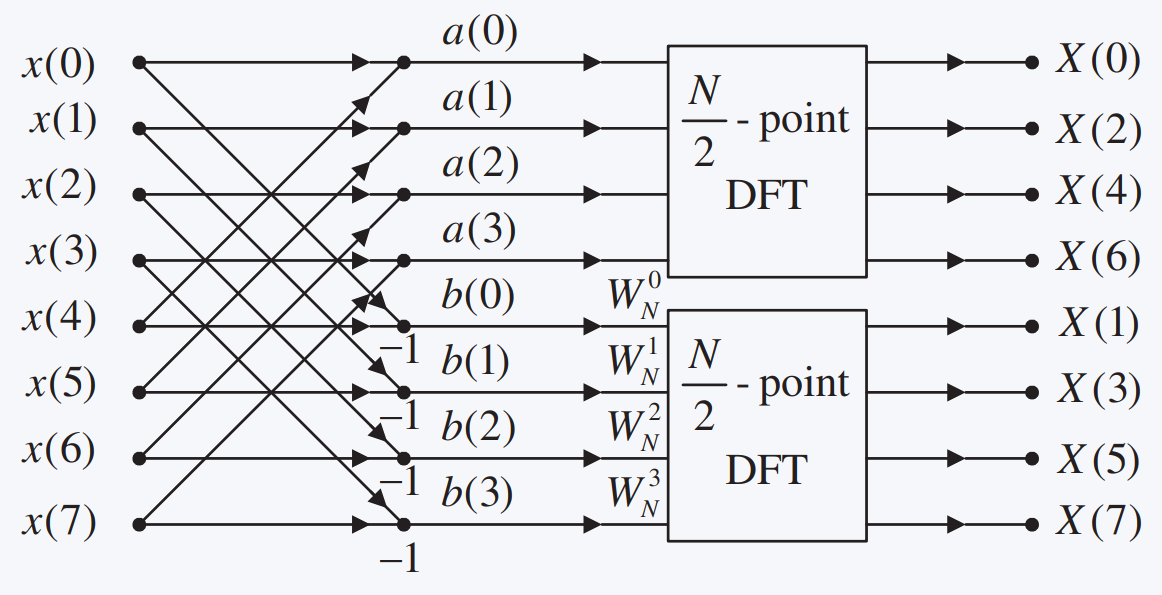
\includegraphics[width=0.6\textwidth]{figures/dif1.png}
    \end{figure}
\end{frame}

\begin{frame}{DIF 8-Point FFT: Full Algorithm}
    \begin{itemize}
        \item Expanding the layers gives the full 8-point DIF structure.
        \item Here inputs are in \textbf{natural} order, while outputs emerge in \textbf{bit-reversed} order.
    \end{itemize}
    \vspace{0.1cm}
    \begin{center}
        \begin{figure}
            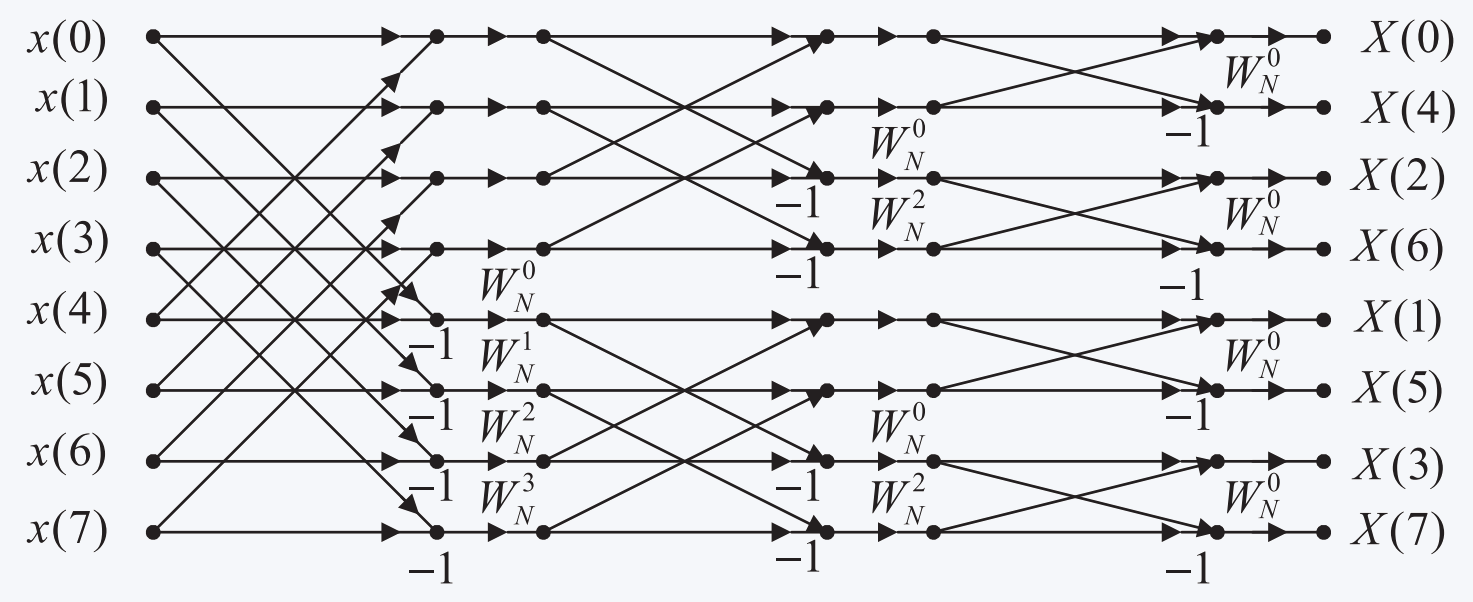
\includegraphics[width=0.7\textwidth]{figures/dif2.png}
        \end{figure}
    \end{center}
\end{frame}

\begin{frame}{Why Zero-Pad? The Practical Necessity}
    \begin{insightbox}{The Radix-2 Requirement}
        Radix-2 FFT algorithms require the sequence length $N$ to be exactly a \textbf{power of 2} ($N = 2^m$).
    \end{insightbox}

    \vspace{0.3cm}
    \textbf{The Problem:}
    \begin{itemize}
        \item Real-world data often consists of $M$ samples, where $M$ is \textbf{not} a power of 2.
        \item If we restrict ourselves to $M$ samples, we are stuck with the slow $O(M^2)$ naive DFT!
    \end{itemize}

    \vspace{0.3cm}
    \textbf{The Solution: Zero-Padding}
    \begin{itemize}
        \item We simply append zeros until we reach the next power of 2: $N = 2^{\lceil \log_2 M \rceil}$.
        \item \textbf{Bonus:} Zero-padding interpolates the spectrum, giving a smoother visualization without altering the true frequency content $X(e^{j\omega})$.
        \item \textbf{However,} if used for periodic $x[n]$, zero-padding changes the period and shape of the periodic signal.
        \item Can we do FFT without zero-padding?
    \end{itemize}
\end{frame}

\end{document}
